\chapter{Sensores}
\label{sec_sensores}

A equipe utiliza dois sensores no projeto: um eletromagnético digital, Bússola; e um ótico, Câmera. O primeiro fornece informação de orientação do robô e o segundo informações visuais do ambiente.

\section{Bússola}
\label{sec_bussola}

A bússola utilizada no projeto é a \textit{Dinsmore Sensor Modelo \# 1490} \cite{bussola}, emprestada à equipe pelo professor Hugo Vieira.

Foi necessário construir um \textit{shield} para conectá-la ao \textit{Arduíno}. O circuito utilizado é apresentado na figura \ref{sen_fig01} e foi baseado no trabalho do \textit{Autonomous Vehicle Team} do \textit{College of New Jersey} \cite{newjersey}.

Internamente a bússola funciona como um transistor coletor aberto NPN e fornece sinais 0 ou 5V, TTL, \cite{bussola}, captados nos catodos dos diodos, para as entradas digitais do \textit{Arduíno}, sendo alimentada com 5V através do \textit{Arduíno} também.

\begin{figure}[h!]
    \center
    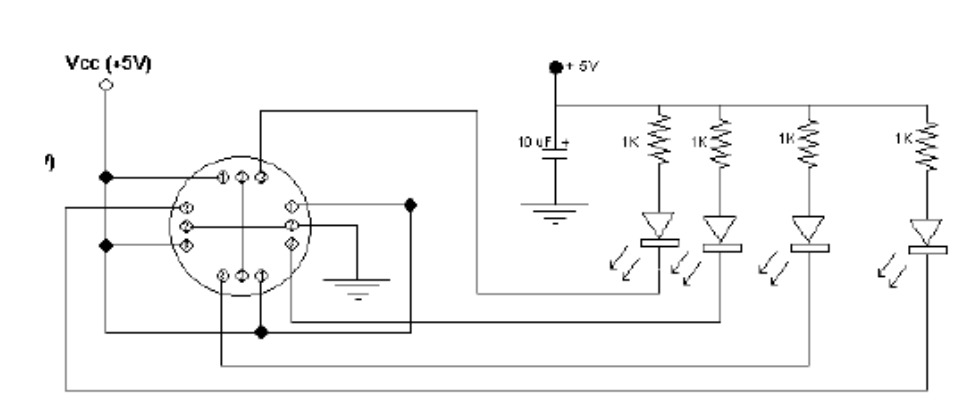
\includegraphics[scale=0.4]{imagens/circuito_bussola.png}
    \caption{Circuito Eletrônico - Bússola}
    \label{sen_fig01}
\end{figure}

A combinação dos quatro sinais fornecidos pela bússola fornece sua orientação com uma precisão de 45 graus, \textit{i.e.}, há oito estados possíveis para a bússola. 

A combinação entre esses estados e sua representação são apresentados na Tabela \ref{sen_tbl01}. As combinações de \textit{bits} que não representam um estado válido não são apresentadas.

\begin{table}[h!]
    \centering
    \begin{tabular}{|c|c|c|c|c|c|} \hline
        \textbf{Sinal 1} & \textbf{Sinal 2} & \textbf{Sinal 3} & \textbf{Sinal 4} & \multicolumn{2}{|c|}{\textit{Direção}} \\ \hline
        0 & 0 & 0 & 1 & W & Oeste \\ \hline
        0 & 0 & 1 & 0 & S & Sul \\ \hline
        0 & 0 & 1 & 1 & SW & Sudoeste \\ \hline
        0 & 1 & 0 & 0 & E & Leste \\ \hline
        0 & 1 & 1 & 0 & SE & Sudeste \\ \hline
        1 & 0 & 0 & 0 & N & Norte \\ \hline
        1 & 0 & 0 & 1 & NW & Noroeste \\ \hline
        1 & 1 & 0 & 0 & NE & Nordeste \\ \hline
    \end{tabular}
    \caption{Acionamento dos Motores}
    \label{sen_tbl01}
\end{table}

\section{Câmera}
\label{sec_camera}
